\documentclass[14pt,a4paper]{article}

\usepackage[russian]{babel}
\usepackage{hyperref} % for hyper links
\usepackage{indentfirst}
\usepackage{float} % for float option H
\usepackage{geometry}
\usepackage{graphicx} % for imgs
\usepackage{verbatim} % fore including .txt files
\usepackage{longtable}

\setlength{\parindent}{0.5cm}  % Установка отступа для абзацев
\geometry{top=2cm, bottom=2cm, left=1.5cm, right=1.5cm}


\renewcommand{\thesubsection}{\arabic{subsection}} % Задания нумерации для
% \subsection

\begin{document}
% Титульный лист
\begin{titlepage}
  \begin{center}
    {\large\scshape\bfseries
    МИНИСТЕРСТВО НАУКИ И ВЫСШЕГО ОБРАЗОВАНИЯ РОССИЙСКОЙ ФЕДЕРАЦИИ\\
    ФЕДЕРАЛЬНОЕ ГОСУДАРСТВЕННОЕ АВТОНОМНОЕ ОБРАЗОВАТЕЛЬНОЕ УЧРЕЖДЕНИЕ ВЫСШЕГО
    ОБРАЗОВАНИЯ\\
    «СЕВЕРО-КАВКАЗСКИЙ ФЕДЕРАЛЬНЫЙ УНИВЕРСИТЕТ»\\
    ФАКУЛЬТЕТ МАТЕМАТИКИ И КОМПЬЮТЕРНЫХ НАУК ИМЕНИ ПРОФЕССОРА Н.И.ЧЕРВЯКОВА}
    \vfill
    \Large{\textbf{ЛАБОРАТОРНАЯ РАБОТА №18}}\\[2mm]
    \large{Алгоритмизация и программирование}\\[6mm]
    \large{\textbf{Вектор}}\\[20mm]
  \end{center}
  \begin{flushright}
    \large{
      \textbf{Выполнил студент:}\\
      Сивко Иван Андреевич\\
      студент 2 курса\\
      группа ПМИ-б-о-23-2,\\
      направление подготовки 01.03.02\\[5mm]
      \textbf{Проверил:}\\
      Ассистент кафедры вычислительной\\
      математики и кибернетики, к.ф.-м.н.,\\
      Черкашина Анастасия Андреевна}
  \end{flushright}
  \vfill
  \centerline{ \the\year\ г. }
\end{titlepage}

% Осноновная часть
\centerline{\large\textbf{Вариант 9}}
\large{\textbf{Цель:}}
\begin{small}
  \begin{itemize}
    \item Совершенствование навыков разработки программ в среде
      программирования MS VStudio
    \item Совершенствование навыков в программировании с использованием векторов
    \item Исследование процесса формирования вектора
    \item Исследование операций с элементами векторов
  \end{itemize}
\end{small}
\section*{Задание 1}
\subsection{Условие:}
Используя полученную при выполнении лабораторной работы 10 в Задании II
программу, реализовать возможность сохранения и обработки данных с
использованием вектора.\\
{\small\textbf{Условие задания 2 лабораторной 10:}\\
\textit{
  В одномерном массиве, состоящем из n вещественных элементов, вычислить:
  \begin{itemize}
    \item максимальный по модулю элемент массива;
    \item преобразовать массив таким образом, чтобы элементы, равные нулю,
      располагались после всех остальных.
  \end{itemize} } }
\subsection{Алгоритм / Мат. модель}
Программа инициализирует а затем заполняет вектор размера введенного
пользователем числами от -100 до 100 затем выводит этот вектор,
после выводит максимальный элемент массива и преобразует его таким
образом, чтобы элементы, равные нулю, располагались после всех остальных.
\begin{enumerate}
  \item ввод размера для векторв \texttt{vec} (в переменную \texttt{size} типа
    \textit{size\_t (aka unsigned long)})
  \item инициализация вектора \texttt{vec} типа \textit{double}
  \item Заполнеине вектора лучайными значениями в пределах от -100 до 100
  \item вывод вектора \texttt{vec} после заполнения и вывод максимального
    по абсалютной велечине значения вектора
  \item перемещения всех 0 в \texttt{vec} в конец вектора
  \item вывод вектора \texttt{vec} после перемещения всех 0 в конец вектора
\end{enumerate}
\begin{table}[H]
  \centering
  \begin{tabular}{|l|l|p{8cm}|} \hline
    \textbf{Название} & \textbf{Тип} & \textbf{Описание} \\ \hline
    \multicolumn{3}{|l|}{\textbf{Классы и структуры}} \\ \hline
    Randgen & class & Генератор случайных чисел с различными распределениями. \\ \hline
    \multicolumn{3}{|l|}{\textbf{Переменные-члены Randgen}} \\ \hline
    state & std::mt19937 & Генератор случайных чисел Mersenne Twister, инициализированный функцией helpInitMt. \\ \hline
    \multicolumn{3}{|l|}{\textbf{Функции-члены Randgen}} \\ \hline
    helpInitMt() & static std::mt19937 & Инициализирует генератор случайных чисел с использованием текущего времени и случайных значений от std::random\_device. \\ \hline
    get<T>(const T\&, const T\&) & static T & Генерирует случайное число типа T в указанном диапазоне (целое или вещественное). \\ \hline
    \multicolumn{3}{|l|}{\textbf{Другие функции}} \\ \hline
    abs(T n) & constexpr T & Возвращает модуль числа n. \\ \hline
    swap(T\& a, T\& b) & void & Обменивает значения переменных a и b. \\ \hline
    operator<< & std::ostream\& & Перегрузка оператора << для вывода элементов вектора std::vector<T> в поток. \\ \hline
    initVecWithRandomNum & void & Инициализирует вектор случайными числами (используя функцию генерации случайных чисел, по умолчанию Randgen::get). \\ \hline
    findAbsMax & const T\& & Находит и возвращает элемент вектора с наибольшим абсолютным значением. \\ \hline
    moveZerosToTheEnd & void & Перемещает все нулевые элементы вектора в конец, сохраняя порядок остальных элементов. \\ \hline
    \multicolumn{3}{|l|}{\textbf{Переменные main}} \\ \hline
    size & size\_t & Количество элементов вектора, вводимое пользователем. \\ \hline
    vec & std::vector<double> & Вектор вещественных чисел, инициализируемый случайными значениями. \\ \hline
  \end{tabular}
  \caption{Переменные функции и классы используемы при решении задачи}
  \label{tabel:1}
\end{table}
% \newpage
\subsection{Диаграмма:}
\begin{figure}[H]
  \centering
  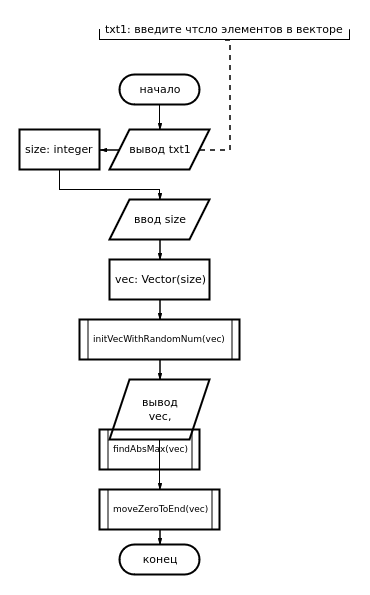
\includegraphics[width=0.8\textwidth]{data/diagram18_1.png}
\end{figure}
% \newpage
\subsection{Код:}
\verbatiminput{data/task18_1.cpp}
\href{https://raw.githubusercontent.com/John1400800/stuff/refs/heads/main/c_learning/home_works/task18_1.cpp}{source code}
\subsection{Результат работы программы:}
\begin{figure}[H]
  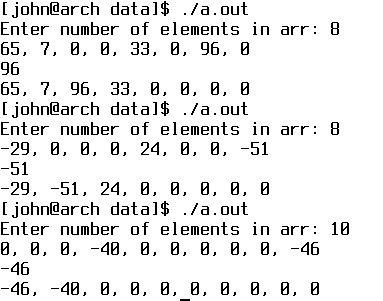
\includegraphics[width=0.8\textwidth]{data/demo18_1.png}
\end{figure}
\section*{Задание 2}
\setcounter{subsection}{0}
\subsection{Условие:}
\begin{enumerate}
  \item Разработать соответствующую варианту программу с использованием
    имеющегося описания, отладить ее и перерешать с использованием векторов.
  \item Подготовить набор тестов, подтверждающих правильность работы программы.
  \item Оформить отчет, включив в него постановку задачи коды программ и
    результаты их работы.
\end{enumerate}
\begin{quote}
  \begin{small}
    Задано описание:\\[1mm]

    \textsl{
      typedef float* Vector[100];\\
      Vector x;
    }

    Считая, что все элементы вектора x отличны от \textsl{NULL}, описать

    \begin{itemize}
      \item процедуру del(x), которая в векторе x все ссылки указывающие на
        повторяющиеся элементы заменяет значением NULL;
      \item процедуру Inp(x) – формирования вектора x;
      \item процедуру Out(x) – вывода чисел, на которые ссылаются элементы
        вектора x отличные от NULL.
    \end{itemize}
  \end{small}
\end{quote}
\subsection{Алгоритм / Мат. модель}
Программа использует динамическую структуру данных для работы с векторами
указателей. Она инициализирует вектор случайными числами, удаляет повторяющиеся
элементы, заменяя их на \texttt{nullptr}, и выводит оставшиеся элементы.
\begin{enumerate}
  \item \textbf{Инициализация вектора:} Создаётся вектор \texttt{vec1} типа
    \textsl{float*[100]} (размером 100), элементы которого являются указателями на тип
    \textsl{float}.
  \item \textbf{Формирование вектора:} Вектор \texttt{vec1} заполняется случайными
    числами от -100 до 100 или последовательностью чисел от 0 до 9 с помощью
    функции \texttt{fillOneToNine} или \texttt{fillRandom}.
  \item \textbf{Вывод начального состояния:} Выводится содержимое вектора
    \texttt{vec1} с использованием перегруженного operator\texttt{<<}, который
    выводит только значения, на которые указывают ненулевые указатели.
  \item \textbf{Удаление повторяющихся элементов:} Функция \texttt{del(vec)}
    заменяет все ссылки на повторяющиеся элементы вектора \texttt{vec1} на
    \texttt{nullptr}.
  \item \textbf{Вывод после обработки:} Выводится содержимое вектора после
    удаления повторяющихся элементов.
  \item \textbf{Реализация с помощью std::vector:} Аналогичные действия
    выполняются с использованием контейнера \textsl{std::vector<float*>}
\end{enumerate}
\begin{table}[H]
  \centering
  \resizebox{\textwidth}{!}{
    \begin{tabular}{|l|l|p{8cm}|} \hline
      \textbf{Название} & \textbf{Тип} & \textbf{Описание} \\ \hline
      \multicolumn{3}{|l|}{\textbf{Классы и структуры}} \\ \hline
      Randgen & Randgen & Генератор случайных чисел с различными распределениями. \\ \hline
      Vector & template T*[N] & Шаблон массива указателей фиксированного размера. \\ \hline
      Vec100PtrtoFloat & Vector<float, 100> & Шаблон массива указателей на float размера 100. \\ \hline
      \multicolumn{3}{|l|}{\textbf{Переменные-члены Randgen}} \\ \hline
      state & static std::mt19937 & Генератор случайных чисел Mersenne Twister, инициализированный функцией helpInitMt. \\ \hline
      \multicolumn{3}{|l|}{\textbf{Функции-члены Randgen}} \\ \hline
      helpInitMt() & static std::mt19937 & Инициализирует генератор случайных чисел с использованием текущего времени и случайных значений от std::random\_device. \\ \hline
      get<T>(const T\&, const T\&) & static T & Генерирует случайное число типа T в указанном диапазоне (целое или вещественное). \\ \hline
      \multicolumn{3}{|l|}{\textbf{Шаблонные функции}} \\ \hline
      del(Vector<T, N>\&)   & void & Удаляет дубликаты указателей в массиве фиксированного размера. \\ \hline
      del(std::vector<T>\&) & void & Удаляет дубликаты указателей в векторе std::vector. \\ \hline
      operator<<(std::ostream\&, const Vector<T, N>\&) & std::ostream\& & Перегрузка оператора << для вывода массива указателей фиксированного размера. \\ \hline
      operator<<(std::ostream\&, const std::vector<T>\&) & std::ostream\& & Перегрузка оператора << для вывода std::vector указателей. \\ \hline
      operator>>(std::istream\&, Vector<T, N>\&) & std::istream\& & Перегрузка оператора >> для ввода массива указателей фиксированного размера. \\ \hline
      operator>>(std::istream\&, std::vector<T>\&) & std::istream\& & Перегрузка оператора >> для ввода std::vector указателей. \\ \hline
      fillRandom(Vector<T, N>\&, Randgen::RandomFunc<T>) & void & Заполняет массив указателей фиксированного размера случайными числами. \\ \hline
      fillRandom(std::vector<T>\&, Randgen::RandomFunc<T>) & void & Заполняет std::vector указателей случайными числами. \\ \hline
      fillOneToNine(Vector<T, N>\&) & void & Заполняет массив указателей фиксированного размера числами от 0 до 9 циклично. \\ \hline
      fillOneToNine(std::vector<T>\&) & void & Заполняет std::vector указателей числами от 0 до 9 циклично. \\ \hline
      \multicolumn{3}{|l|}{\textbf{Переменные main}} \\ \hline
      vec1 & Vec100PtrtoFloat & Массив указателей на float фиксированного размера 100, заполняемый числами от 0 до 9. \\ \hline
      vec2 & std::vector<float*> & Вектор указателей на float, заполняемый числами от 0 до 9. \\ \hline
    \end{tabular}
  }
  \caption{Переменные, функции и классы, используемые в программе}
  \label{tabel:1}
\end{table}
\subsection{Диаграмма:}
\begin{figure}[H]
  \centering
  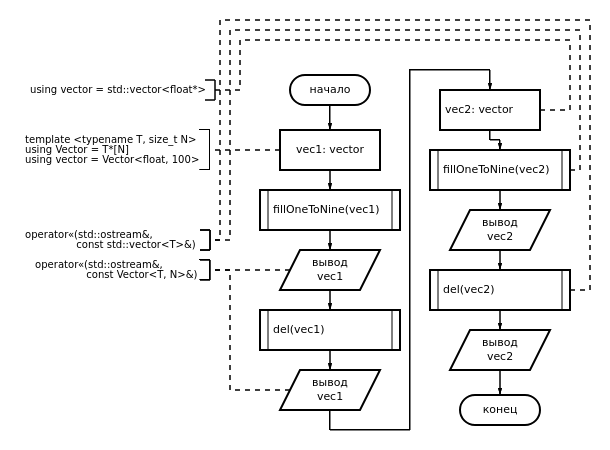
\includegraphics[width=0.8\textwidth]{data/diagram18_2.png}
\end{figure}
\subsection{Код:}
\verbatiminput{data/task18_2.cpp}
\href{https://raw.githubusercontent.com/John1400800/stuff/refs/heads/main/c_learning/home_works/task18_2.cpp}{source code}
\subsection{Результат работы программы:}
\begin{figure}[H]
  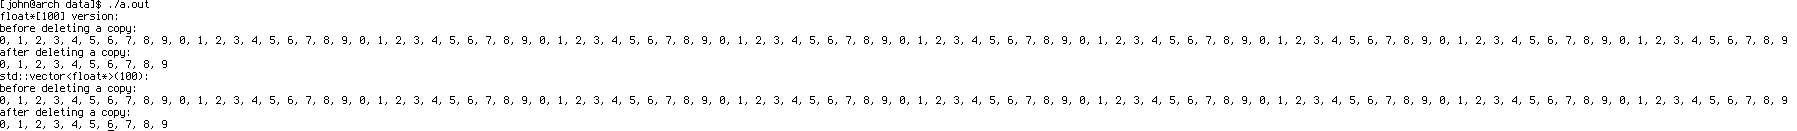
\includegraphics[width=0.9\textwidth]{data/demo18_2.png}
\end{figure}
\section*{Задание 3}
\textsl{В соответствии с вариантом написать и отладить программу, используя структуру данных: a) массив ссылок на строки; b) вектор строк;}\\
\setcounter{subsection}{0}
\subsection{Условие:}
Используя данное представление текста, описать
\begin{itemize}
  \item функцию find(Т, с), определяющую, сколько раз литера с входит в текст Т;
  \item функцию void  Inp(Т), считывающую из входного файла последовательность
    литер до первой * ( - символ окончания текста) и формирующую из них текст Т
    (последнюю строку, если надо, дополнить пробелами);
  \item функцию void  out(Т), печатающую построчно текст Т.
\end{itemize}
{\large\textbf{a)}}
\subsection{Алгоритм / Мат. модель}
Программа использует динамическую структуру данных для работы с текстом,
хранящим строки, и анализирует их на наличие символов. Она читает строки из
файла, делит их на части заданной длины, подсчитывает количество вхождений
заданного символа и выводит результат. Также освобождает динамическую память,
используемую для хранения строк.
\begin{enumerate}
  \item \textbf{Инициализация структуры данных:} Создаётся структур
    \texttt{TextLines}, которая содержит:
    \begin{itemize}
      \item \texttt{lines} — динамический массив указателей на строки типа \textsl{char*},
      \item \texttt{numLines} — количество строк в массиве,
      \item \texttt{maxLines} — максимальный размер массива строк.
    \end{itemize}
  \item \textbf{Чтение текста из файла:} Функция \texttt{readTextFromFile}
    читает содержимое файла и разбивает строки на части длиной не более
    \texttt{MAX\_LINE\_LENGTH} символов с учетом пробелов. Для каждой части
    выделяется память, и она добавляется в массив строк.
  \item \textbf{Перераспределение памяти:} Если количество строк превышает
    текущий лимит \texttt{maxLines}, то выполняется увеличение размера массива
    в два раза.
  \item \textbf{Подсчёт вхождений символа:} Функция \texttt{countOccurrences}
    подсчитывает количество вхождений заданного символа \texttt{searchChar} в
    строках, используя два вложенных цикла — по строкам и по символам внутри
    каждой строки.
  \item \textbf{Вывод строк:} Функция \texttt{printTextLines} выводит каждую
    строку с её индексом.
  \item \textbf{Освобождение памяти:} Функция \texttt{freeTextLines}
    освобождает всю выделенную память, связанную с текстовыми строками, и
    обнуляет указатели на массив строк.
  \item \textbf{Реализация через командную строку:} Программа получает имя
    файла для чтения и, если указано, символ для подсчёта его вхождений.
    Результат выводится в консоль.
\end{enumerate}
\begin{table}[H]
  \centering
  \resizebox{\textwidth}{!}{
    \begin{tabular}{|l|l|p{8cm}|} \hline
      \textbf{Название} & \textbf{Тип} & \textbf{Описание} \\ \hline
      \multicolumn{3}{|l|}{\textbf{Структуры}} \\ \hline
      TextLines & struct & Структура для хранения текста, содержащая динамический массив строк \texttt{char*}, количество строк \texttt{numLines} и максимальное количество строк \texttt{maxLines}. \\ \hline
      \multicolumn{3}{|l|}{\textbf{Функции}} \\ \hline
      readTextFromFile() & bool & Читает текст из файла, разбивает его на строки длиной не более \texttt{maxLineLength}, и сохраняет их в структуре \texttt{TextLines}. \\ \hline
      countOccurrences() & size\_t & Подсчитывает количество вхождений символа \texttt{searchChar} во всех строках, сохранённых в структуре \texttt{TextLines}. \\ \hline
      freeTextLines() & void & Освобождает память, выделенную для строк в структуре \texttt{TextLines}, и обнуляет указатели. \\ \hline
      printTextLines() & void & Выводит все строки из структуры \texttt{TextLines} на экран с их индексами. \\ \hline
      \multicolumn{3}{|l|}{\textbf{Переменные main}} \\ \hline
      filename & char[256] & Строка для хранения имени файла, которое будет считано с консоли или из командной строки. \\ \hline
      searchChar & char & Символ, количество вхождений которого подсчитывается в тексте. \\ \hline
      file & FILE* & Указатель на файл, который открывается для чтения. \\ \hline
      lines & TextLines & Структура, в которой сохраняются строки, прочитанные из файла. \\ \hline
    \end{tabular}
  }
  \caption{Переменные, функции и структуры, используемые в программе}
  \label{tabel:1}
\end{table}
\subsection{Диаграмма:}
\begin{figure}[H]
  \centering
  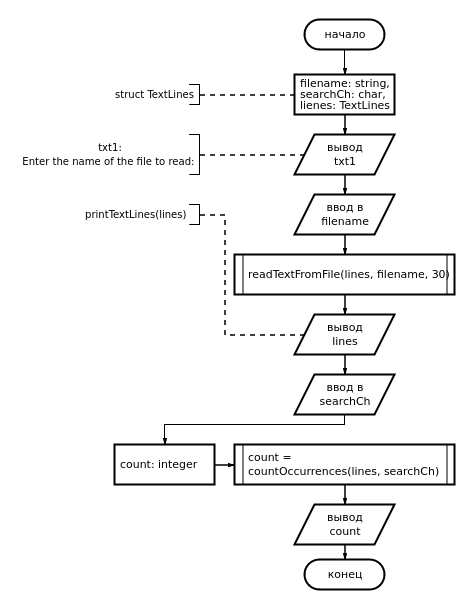
\includegraphics[width=0.8\textwidth]{data/diagram18_3a.png}
\end{figure}
\subsection{Код:}
\verbatiminput{data/task18_3a.c}
\href{https://raw.githubusercontent.com/John1400800/stuff/refs/heads/main/c_learning/home_works/task18_3a.c}{source code}
\subsection{Результат работы программы:}
\begin{figure}[H]
  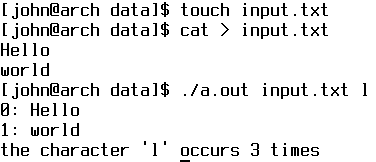
\includegraphics[width=0.4\textwidth]{data/demo18_3a.png}
\end{figure}
\newpage
{\large\textbf{b) вариант с векторами}}
\setcounter{subsection}{0}
\subsection{Алгоритм / Мат. модель}
Программа читает содержимое текстового файла, форматирует его строки, заменяя
пробелы на новые строки, и подсчитывает количество вхождений определённого
символа в текст.
\begin{enumerate}
  \item \textbf{Инициализация переменных:}\\
    Программа инициализирует несколько переменных
    \begin{itemize}
      \item \texttt{filename} - строка для хранения имени файла, которое вводит
        пользователь.
      \item \texttt{searchSymbol} - символ, количество вхождений которого нужно
        подсчитать, вводится пользователем.
    \end{itemize}
  \item \textbf{Чтение файла:}
    \begin{itemize}
      \item Функция \texttt{readFile} открывает файл с именем, переданным
        пользователем в качестве параметра.
      \item Если файл не удаётся открыть, выбрасывается исключение с сообщением
        об ошибке.
      \item Если файл открыт успешно, его содержимое считывается и возвращается
        как строка.
    \end{itemize}
  \item \textbf{Форматирование текста::}
    \begin{itemize}
      \item Функция \texttt{strWrap} форматирует текст, заменяя пробелы на символы новой
        строки, если длина строки превышает максимальное значение (\texttt{maxStrLen}).
      \item Программа перезаписывает текст с разбивкой по строкам, где
        максимально возможная длина строки — 30 символов.
      \item Это достигается путём нахождения последнего пробела в строке,
        который будет заменён на новую строку, если длина текущей строки
        превышает заданный лимит.
    \end{itemize}
  \item \textbf{Подсчёт вхождений символа:}
    \begin{itemize}
      \item Функция \texttt{countOccurrences} подсчитывает количество вхождений символа
        \texttt{searchSymbol} в строке, переданной ей как параметр.
      \item Для каждого символа строки, если он совпадает с \texttt{searchSymbol}, счётчик увеличивается.
    \end{itemize}
  \item \textbf{Вывод результатов:}
    \begin{itemize}
      \item Программа выводит отформатированный текст из файла.
      \item Затем выводится количество вхождений символа, введённого пользователем, в этот текст.
    \end{itemize}
\end{enumerate}
\begin{table}[H]
  \centering
  \resizebox{\textwidth}{!}{
    \begin{tabular}{|l|l|p{8cm}|} \hline
      \textbf{Название} & \textbf{Тип} & \textbf{Описание} \\ \hline
      \multicolumn{3}{|l|}{\textbf{Типы данных}} \\ \hline
      exitState & enum & Перечисление, определяющее возможные состояния завершения программы: FAILURE (false) и SUCCESS (true). \\ \hline
      \multicolumn{3}{|l|}{\textbf{Функции}} \\ \hline
      readFile() & std::string & Читает содержимое файла и возвращает его в виде строки. Выбрасывает исключение в случае ошибки. \\ \hline
      strWrap() & void & Форматирует строку, разбивая её на подстроки длиной не более maxStrLen, заменяя пробелы на символы новой строки. \\ \hline
      countOccurrences() & size\_t & Подсчитывает количество вхождений символа search в строке str. \\ \hline
      \multicolumn{3}{|l|}{\textbf{Переменные main}} \\ \hline
      filename & std::string & Строка для хранения имени файла, которое вводит пользователь. \\ \hline
      searchSymbol & char & Символ для поиска, который вводит пользователь. \\ \hline
      fileContent & std::string & Строка для хранения содержимого файла, считанного функцией readFile(). \\ \hline
      file & std::ifstream & Поток для чтения файла, используемый в функции readFile(). \\ \hline
    \end{tabular}
  }
  \caption{Переменные, функции и константы, используемые в программе}
  \label{tabel:1}
\end{table}
\subsection{Диаграмма:}
\begin{figure}[H]
  \centering
  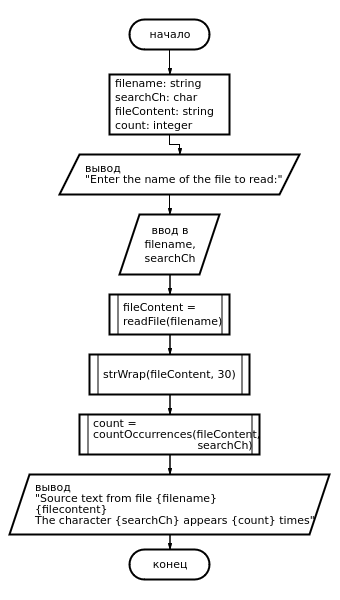
\includegraphics[height=0.5\textheight]{data/diagram18_3b.png}
\end{figure}
\subsection{Код:}
\verbatiminput{data/task18_3b.cpp}
\href{https://raw.githubusercontent.com/John1400800/stuff/refs/heads/main/c_learning/home_works/task18_3b.cpp}{source code}
\subsection{Результат работы программы:}
\begin{figure}[H]
  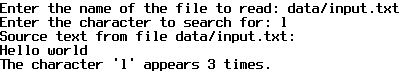
\includegraphics[width=0.5\textwidth]{data/demo18_3b.png}
\end{figure}
\end{document}
